\documentclass[a4paper,10pt]{article}
\usepackage[left=0.75in,top=1.3in,right=0.75in,bottom=0.6in]{geometry} 
\usepackage{multicol}
\usepackage[latin1]{inputenc}
\usepackage[T1]{fontenc}
%\usepackage[francais]{babel}
\usepackage[english]{babel}
\usepackage{graphicx}
\usepackage{epsfig}

\usepackage{geometry}
\usepackage{caption}
\usepackage{fancyhdr}
%\usepackage{background}
\usepackage{color}
\usepackage{natbib}
%\usepackage{aas_macros}
%\usepackage[maxnames=1,minnames=1]{biblatex}



\title{Note for elementary example for perturbation theory}
%\date{}



\begin{document}

\maketitle

The goal of this example is to show the basic idea of perturbation theory. In fact, perturbation theory is not required to solve this example because an analytic solution exist. But, it will be useful in order to get the idea and compare the simplified solution and the first correction term with the analytic solution. Moreover, as you can see in the notebook, there is also a part to obtain the numerical result which is the real way to generate the 'exact' solution because analytical solution does not exist in general.

\section{First order perturbation}

We start with the differential equation:
\begin{equation}
\label{eq:start}
\frac{dx}{dt} + \frac{1}{\tau}x + \frac{\lambda}{\tau L_0}x^2 = 0,
\end{equation}
were $\tau$ is characteristic time and $L_0$ a characteristic length of the system we describe. We easily know how to solve this equation if $\lambda=0$ and we will use it. In general, we do not have a simple way to find the exact solution of this kind of equations. The idea is, in the case where $\lambda$ is small compare to 1, to look for the the solution with $\lambda=0$ and then correct the solution expanding  the $\lambda$ parameter. At first order of perturbation, the idea is to look for a solution $x_s$ as:
\begin{equation}
\label{eq:form_pt}
x_s(t) = x_0(t) + \lambda\times x_1(t) + \mathcal{O}(\lambda^2)
\end{equation}
where $x_0$ is the solution with $\lambda=0$ and $x_1$ the solution when we conserve only the terms $\mathcal{O}(\lambda)$. The idea is probably still confusing now but will be clear after we solve this example. To do the second order, we have to consider all the terms $\mathcal{O}(\lambda)$ for a adding correction in $\lambda^2 x_2$. We will focus on the first order here.

\subsection{Find $x_0$}

We would like to solve:
\begin{equation}
\frac{dx_0}{dt} + \frac{1}{\tau}x_0 = 0,
\end{equation}
which is the elementary differential equation with exponential solution:
\begin{equation}
\frac{dx_0}{dt} = -\frac{1}{\tau}x_0 \qquad \Rightarrow \qquad x_0(t) = A\exp\left(-\frac{1}{\tau}t\right),
\end{equation}
where $A$ is determined with initial condition. We fix that the system start with $x(t=0)=X_0$. So, fixing $t=0$ to the $x_0$ equation it let directly $A=X_0$. So we have the 0 order solution,
\begin{equation}
x_0(t) = X_0\exp\left(-\frac{1}{\tau}t\right) .
\end{equation}

\subsection{Find $x_1$}
We have found the expression of $x_0$ and we want to find the expression of $x_1$. We have first to use the $x(t)$ form (\ref{eq:form_pt}) in the initial equation (\ref{eq:start}) and keep the first order terms in $\lambda$,
\begin{eqnarray}
\frac{d(x_0 + \lambda x_1 ) }{dt} + \frac{1}{\tau}(x_0 + \lambda x_1 ) + \frac{\lambda}{\tau L_0}(x_0 + \lambda x_1 )^2 &=& 0 \\
\underbrace{\frac{dx_0}{dt}  + \frac{1}{\tau}x_0}_{\equiv 0} +   \lambda\left( \frac{dx_1}{dt}  + \frac{1}{\tau}x_1 \right)+ \frac{\lambda}{\tau L_0}(x_0^2 + \underbrace{2\lambda x_0 x_1}_{\mathcal(O)(\lambda^2)} + \underbrace{\lambda^2x_1^2}_{\mathcal(O)(\lambda^3)} ) &=& 0 \\
 \lambda\left( \frac{dx_1}{dt}  + \frac{1}{\tau}x_1 \right)+ \frac{\lambda}{\tau L_0}x_0^2 &=& 0.
\end{eqnarray}
So, $x_1$ have to be solution of the differential equation:
\begin{equation}
 \lambda\left( \frac{dx_1}{dt}  + \frac{1}{\tau}x_1 \right) = -\frac{\lambda}{\tau L_0}X_0^2\exp\left(-\frac{2}{\tau}t\right),
\end{equation}
where we can simplify by $\lambda$. The way to solve this equation is to find an homogeneous $\bar{x}_1$ solution (\textit{i.e} with right hand side equal to zero) and a particular solution $x_1^p$. Here, both are easy because the right hand side is an exponential. Let me start with the homogeneous solution $\bar{x}_1$,
\begin{eqnarray}
\frac{d\bar{x}_1}{dt}  + \frac{1}{\tau}\bar{x_1} = 0\\
\bar{x}_1(t) = B \exp\left(-\frac{1}{\tau}t\right),
\end{eqnarray}
where we will determine the constant B hereafter. The particular solution  $x_1^p$ is of the same form than the right hand side because it is already an exponential so we are looking for a solution like
\begin{equation}
 x_1^p(t) = C\exp\left(-\frac{2}{\tau}t\right),
\end{equation}
for which we can determine the constant C substituting the form of $x_1^p$ in the initial equation as
\begin{eqnarray}
\frac{d}{dt}C\exp\left(-\frac{2}{\tau}t\right)  + \frac{1}{\tau}C\exp\left(-\frac{2}{\tau}t\right)&=& -\frac{1}{\tau L_0}X_0^2\exp\left(-\frac{2}{\tau}t\right)\\
C\left( -\frac{2}{\tau} + \frac{1}{\tau}  \right) exp\left(-\frac{2}{\tau}t\right) &=&- \frac{1}{\tau L_0}X_0^2\exp\left(-\frac{2}{\tau}t\right)\\
C &=& \frac{X_0^2}{L_0}.
\end{eqnarray}
In order to fix the constant B, we have to remember that we fix the constant A to be sure that $x_0$ to be equal to the initial condition $X_0$. So, by definition, solution $x_0$ is exact at $t=0$ which means that all the corrective term of higher order have to be null at $t=0$. So, we need $x_1(t=0) = \bar{x}_1(t=0) + x_1^p(t=0) = 0$.
\begin{eqnarray}
\bar{x}_1(t=0) + x_1^p(t=0) &=& B +  \frac{X_0^2}{L_0} = 0\\
B &=& - \frac{X_0^2}{L_0}.
\end{eqnarray}
So, the complete solution of $x_1$ is given by
\begin{equation}
x_1 = -\frac{X_0^2}{L_0} \exp\left(-\frac{1}{\tau}t\right) + \frac{X_0^2}{L_0} \exp\left(-\frac{2}{\tau}t\right).
\end{equation}
The final result, substituting the expression of $x_0$ and $x_1$ in equation ()
\begin{equation}
x_s(t) = X_0\exp\left(-\frac{1}{\tau}t\right) +\lambda\left[-\frac{X_0^2}{L_0} \exp\left(-\frac{1}{\tau}t\right) + \frac{X_0^2}{L_0} \exp\left(-\frac{2}{\tau}t\right)\right].
\end{equation}

\begin{figure}[!hp]
\hspace*{-2.1cm}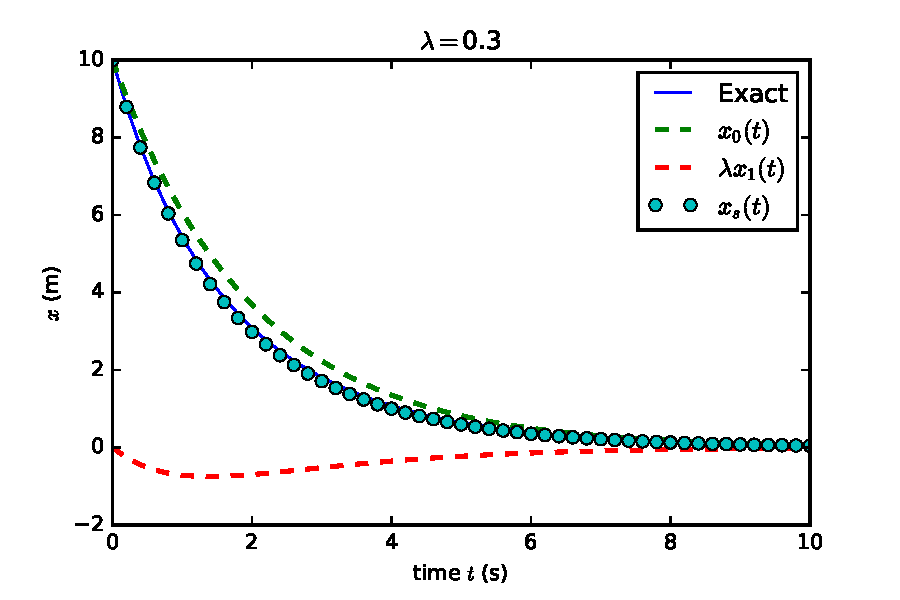
\includegraphics[width=4.5in]{PT_lambda=03.pdf}\hspace*{-1.1cm}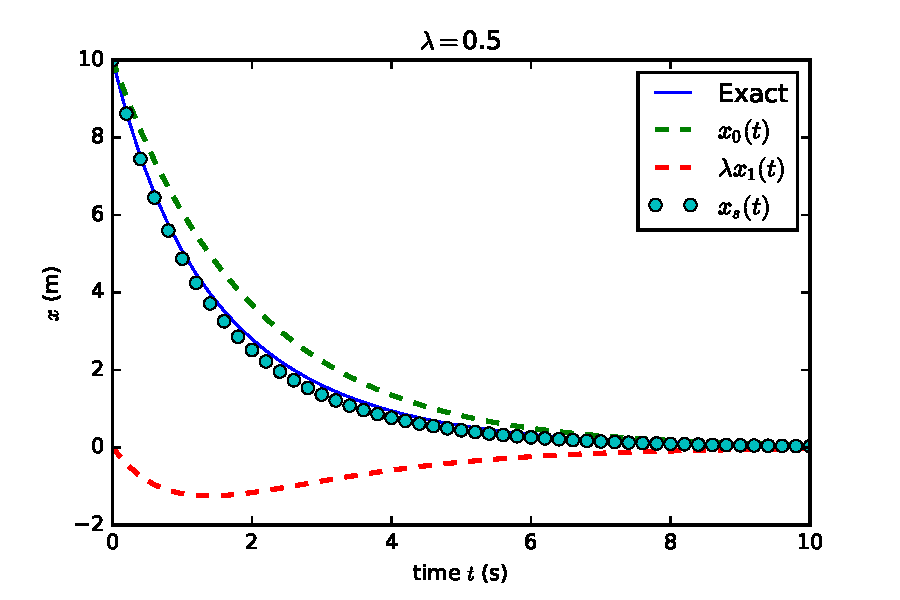
\includegraphics[width=4.5in]{PT_lambda=05.pdf}\\
\hspace*{-2.1cm}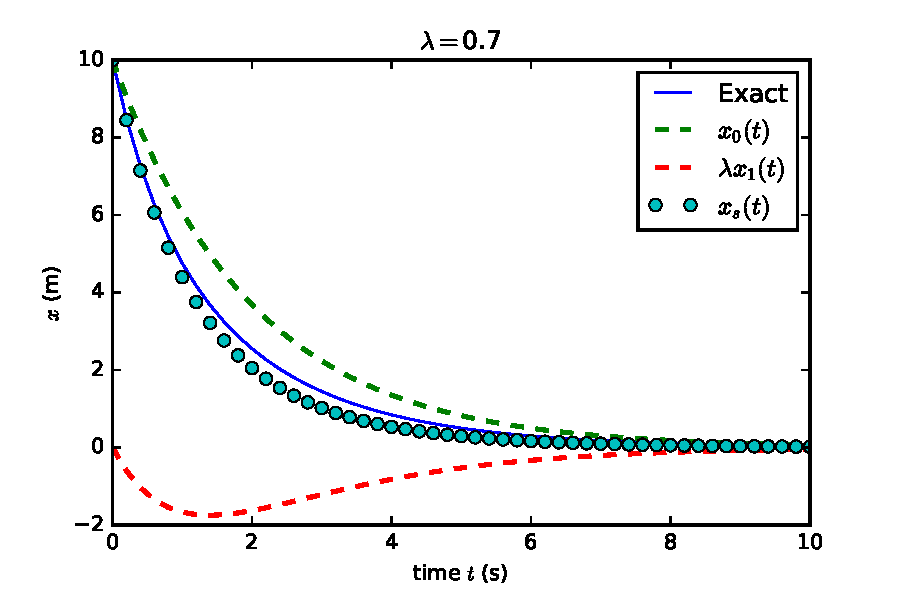
\includegraphics[width=4.5in]{PT_lambda=07.pdf}\hspace*{-1.1cm}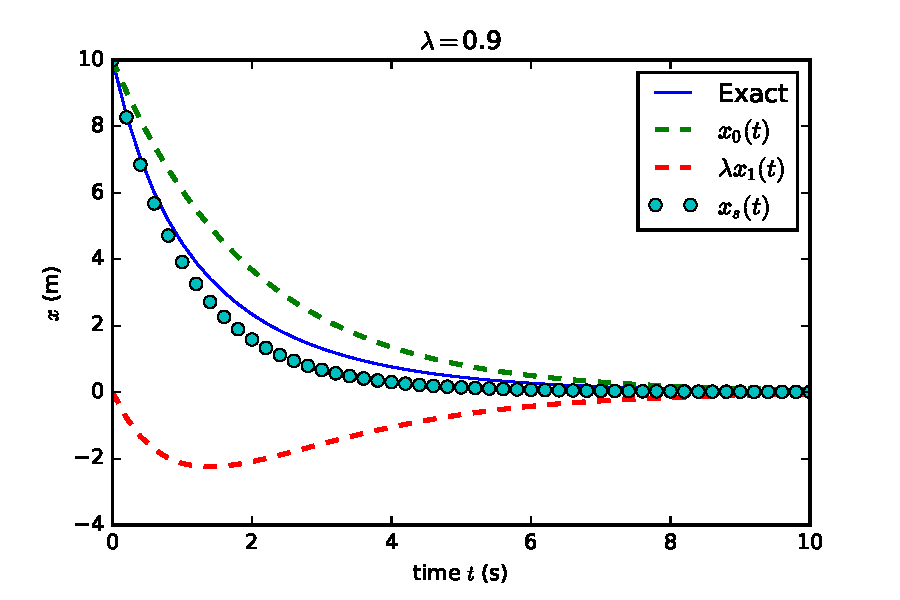
\includegraphics[width=4.5in]{PT_lambda=09.pdf}
\caption{Comparison between the exact solution and the first order perturbation solution for different values of $\lambda$. We can see the correction from the first order perturbative $x_1$. The correction is efficient for low value of $\lambda$. The results are obtained using $X_0=10$m, $L_0=10$m and $\tau=2$s }
\label{default}
\end{figure}

\newpage
\section{Simulation}

As explained above, we normally apply perturbation theory when we do not have a method to obtain the exact analytic solution. We will solve this easy problem using a very simple simulation. We start from the initial condition $X_0=10$m. Then we have to use the equation (\ref{eq:start}) in order to determine the variation $\Delta x$. We have to use $\Delta Q$ rather than $dQ$ because we have to choose a finite step size for $\Delta t$. So, we have to remember it and evaluate the error budget. We have the following system:
\begin{eqnarray}
x(t=0) &=& X_0\\
x(\Delta t) &=& x(0) - \left(  \frac{1}{\tau}x(0) + \frac{\lambda}{\tau L_0}x^2(0) \right)\times \Delta t\\
x(2\Delta t) &=& x(\Delta t) - \left(  \frac{1}{\tau}x(\Delta t) + \frac{\lambda}{\tau L_0}x^2(\Delta t) \right)\times \Delta t\\
\ldots \\
x(k\Delta t) &=& x( (k-1)\Delta t) - \left(  \frac{1}{\tau}x((k-1)\Delta t) + \frac{\lambda}{\tau L_0}x^2((k-1)\Delta t) \right)\times \Delta t
\end{eqnarray}

\begin{figure}[!hp]
\hspace*{-2.1cm}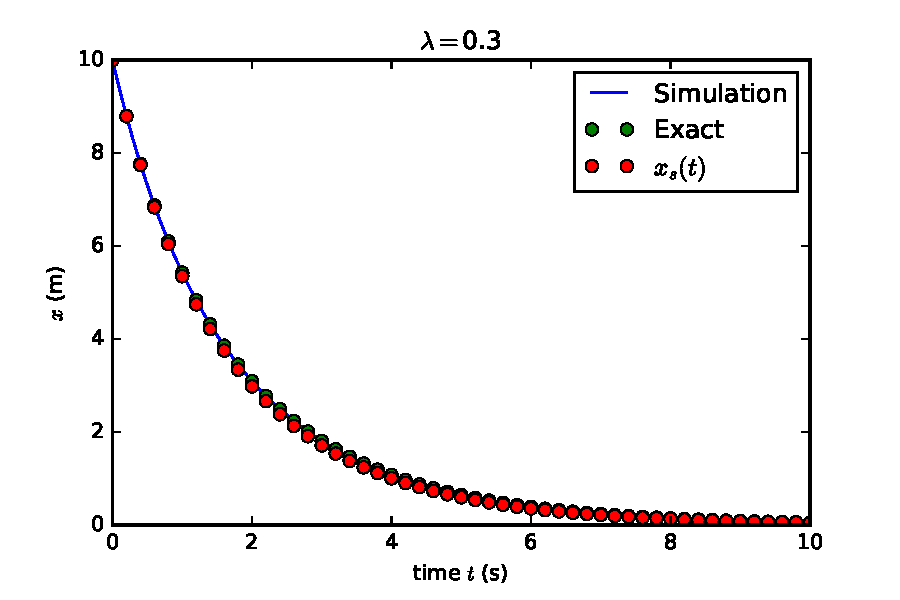
\includegraphics[width=4.5in]{Simus_lambda=03.pdf}\hspace*{-1.1cm}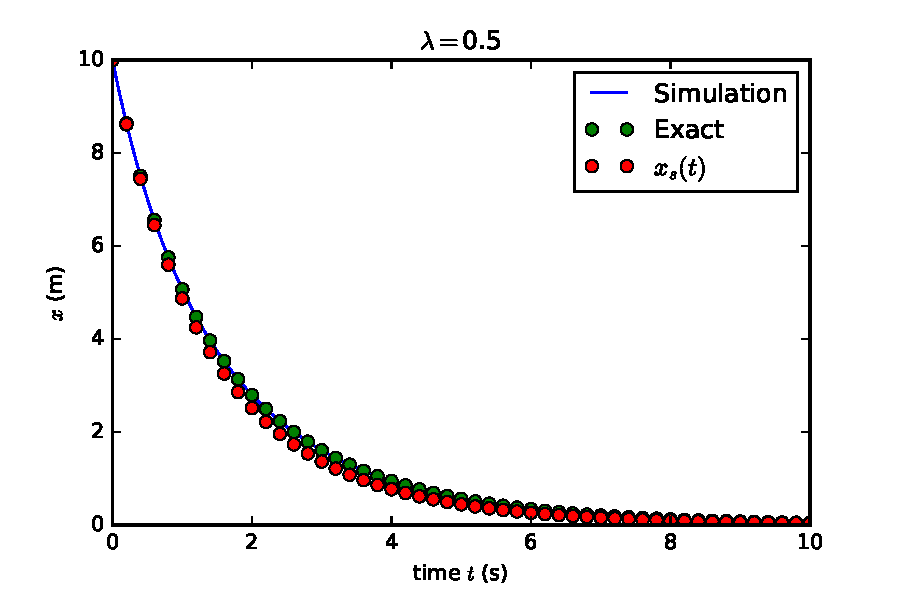
\includegraphics[width=4.5in]{Simus_lambda=05.pdf}\\
\hspace*{-2.1cm}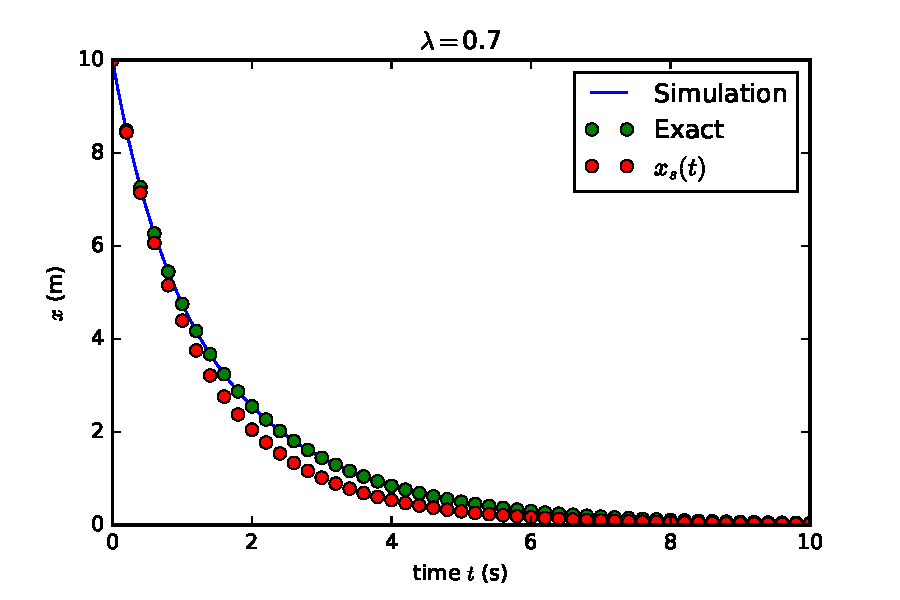
\includegraphics[width=4.5in]{Simus_lambda=07.pdf}\hspace*{-1.1cm}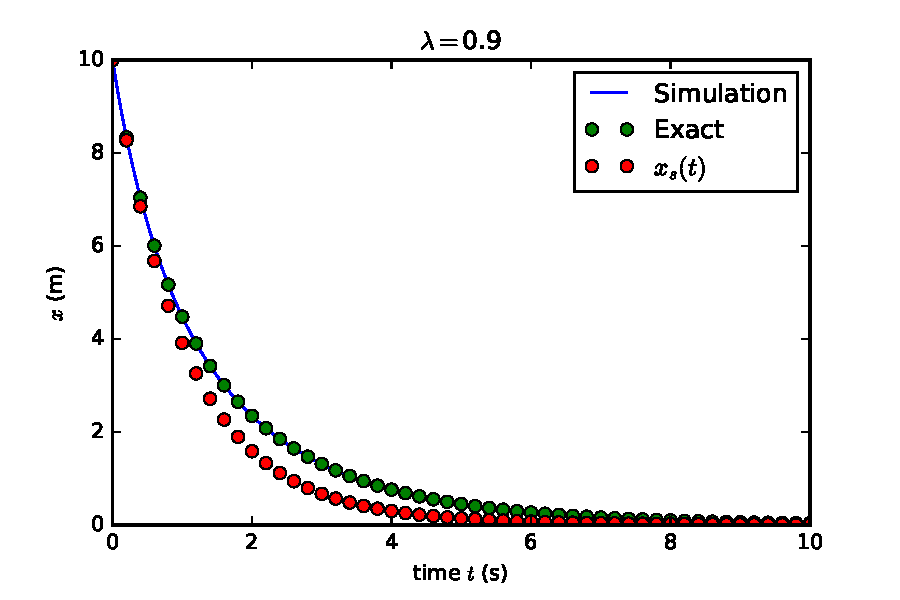
\includegraphics[width=4.5in]{Simus_lambda=09.pdf}
\caption{Comparison between the simulation, the exact solution and the first order perturbation solution for different values of $\lambda$. We can see that the simulation reproduce perfectly the exact solution. The results are obtained using $X_0=10$m, $L_0=10$m and $\tau=2$s }
\label{default}
\end{figure}

\end{document}